\chapter{SWITCH 方式}
\label{sec:switch}
従来の IQ では,空きエントリがあればディスパッチすることができたが,これまで提案した手法では,ディスパッチできるエントリは選択されたセグメントに限定されている.このため,IQ の容量効率が低下するという問題がある.本章では,この問題に対応する手法である SWITCH  方式に関して説明する.\refsec{occupency_reduction}で IQ の容量効率の低下に関して説明した後,\refsec{switch_scheme}で SWITCH 方式に関して説明する.

\begin{figure}[tb]
  \centering
  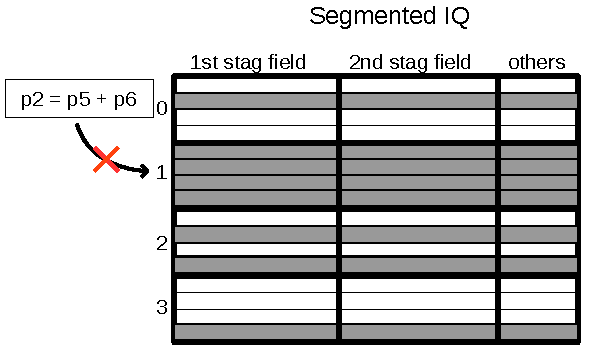
\includegraphics[keepaspectratio, scale=.8]{stall_segmentedIQ}
  \caption{容量効率が低下する例}
  \label{fig:stall_segmentedIQ}
\end{figure}


\section{容量効率の低下}
\label{sec:occupency_reduction}
提案手法には IQ の容量効率が低下するという問題がある.この問題は,IQ の容量効率が重要なプログラムにおいて,性能低下を引き起こす.本節では,容量効率が低下する原因について説明した後,容量効率の低下により性能低下を引き起こすプログラムの特徴に関して説明する.

\subsection{提案手法による容量効率低下の原因}
IQ の容量効率の低下に関して,\fig{stall_segmentedIQ}を用いて説明する.図において,灰色のエントリは命令を保持していることを示している.

図の状態の IQ に,新たに命令 $p2 = p5 + p6$ をディスパッチする場合を考える.この命令のソース・オペランドは両方レディでないとする.この場合,第 1 ソース・タグの下位ビットから第 1 セグメントにディスパッチされることが決定する.しかし,第 1 セグメントに空きエントリはないため,空きが出るまでディスパッチをストールさせ,待ち合わせを行う必要がある.

このように,命令がディスパッチされるセグメントに空きがない場合,他のセグメントに空きがあってもディスパッチできないため,提案手法ではセグメント化されていない IQ と比較して容量効率が低下する.

\subsection{容量効率の低下による性能低下}
プログラムには,性能が IQ の容量に敏感なものとそうでないものとがある~\cite{Ando2019, Kora2013, Sembrant2015}.次の 2 つの特徴のうちいずれかに当てはまるプログラムでは,性能が IQ の容量に敏感なため,与えられた IQ の容量においては,その利用効率が重要である.このため,提案手法による容量効率の低下によって性能が低下する.
\begin{itemize}
  \item \textbf{命令レベル並列性(ILP:Instruction Level Parallelism)}が高いプログラム
  \item \textbf{メモリ・レベル並列性(MLP:Memory Level Parallelism)}が高いプログラム 
\end{itemize}

ILP が高いプログラムでは,IQ に命令をできるだけ多く供給し,より多くの命令を並列に発行できるようにすることで高い性能が得られる.IQ の容量効率が低下すると,並列に発行できる命令数が減少するため,性能が低下する.

MLP が高いプログラムでは,キャッシュ・ミスを生じるできるだけ多くの命令を並列に実行することにより,メモリ・アクセスのレイテンシが実行時間に与える影響を縮小できる.IQ の容量効率が低下すると,並列に処理できるメモリ・アクセスが減少するため,性能が低下する.

これらのことから,ILP もしくは MLP が高い場合には,提案手法による容量効率の低下を最小限に抑える工夫が必要となる.

%5 容量効率の低下への対策:SWITCH 方式
\section{容量効率低下への対策:SWITCH 方式}
\label{sec:switch_scheme}
IQ の容量効率低下による性能低下を抑制する方式として,\textbf{SWITCH} と呼ぶ方式を提案する.SWITCH 方式では,次のようにして性能低下を抑制する.
\begin{itemize}
  \item セグメント選択回路の選択アルゴリズムとして,容量効率は低下するが,タグ比較回数を多く削減できるような選択を行う \textbf{AGGRESSIVE モード} と,タグ比較回数の削減率は低下するが,容量効率が大きく低下しないような選択を行う \textbf{CONSERVATIVE モード} の 2 つを用意する.
  \item 実行プログラムの ILP 及び MLP を一定のインターバルで監視し,ILP もしくは MLP が高いと判断されたなら次のインターバルでは CONSERVATIVE モードでディスパッチし,そうでないなら AGGRESSIVE モードでディスパッチする.
\end{itemize}

本節では,まず 2 つのセグメント選択のアルゴリズムに関して説明を行う.その後,ILP 及び MLP の評価方法と,切り替えアルゴリズムに関して説明する.

\subsection{2 つのセグメント選択アルゴリズム}
\label{sec:two_mode}
SWITCH 方式では,タグ比較回数の削減重視の AGGRESSIVE モードと,容量効率重視の CONSERVATIVE モードの 2 つを適切に切り替えて使用する.各モードには,タグ比較回数の削減と容量効率に関して,\tab{switch_trade_off}に示すトレード・オフの関係がある.それぞれのセグメントの選択方法に関して説明する.

なお, SWITCH 方式はサブ・セグメントと併用が可能である.まず,サブ・セグメントを使用しない場合の AGGRESSIVE 及び CONSERVATIVE のアルゴリズムに関した説明した後,サブ・セグメントと併用する場合のアルゴリズムへと拡張して説明する.

\begin{table}[tb]
  \caption{2 つのセグメント選択モードのトレード・オフ}
  \footnotesize
  \center
   \begin{tabular}{l|c|c} \hline \hline
   モード & タグ比較回数の削減 & 容量効率 \\ \hline
   AGGRESSIVE & ○ & × \\
   CONSERVATIVE & × & ○ \\ \hline
  \end{tabular}
  \label{tab:switch_trade_off}
\end{table}

\subsection{AGGRESSIVE モード(サブ・セグメント不使用)}
AGGRESSIVE モードは,\tab{agg_algorithm}に示した選択アルゴリズムを使用してディスパッチするエントリを決定する.このモードでは,選択されたセグメントに空きがない場合,他のセグメントに空きがあってもディスパッチは行わないため,容量効率が低下する.しかし,セグメント化の利益を最大限利用し,タグ比較回数を大幅に削減できる.

\subsection{CONSERVATIVE モード(サブ・セグメント不使用)}
AGGRESSIVE モードでは,命令のソース・オペランドが両方レディであり,セグメント・インディペンデントとしてディスパッチできる場合以外では,ソース・タグによって選択されるセグメントに空きがない場合にディスパッチをストールさせる.これに対し,CONSERVATIVE モードでは,以下で説明する工夫を行うことによって,このディスパッチのストールを回避し,容量効率の低下を抑制する.
\begin{itemize}
  \item \textbf{両ソース・オペランドともレディでない場合}:\\AGGRESSIVE モードでは第 1 ソース・タグの下位ビットによってセグメントを選択する.選択されたセグメントに空きがない場合,ディスパッチを行わない.これに対して CONSERVATIVE モードでは,第 1 ソース・タグによって選択されたセグメントに空きがない場合には,\textbf{スワップ}~\footnote{\ref{sec:swap}節では,スワップの定義を「第 1 ソース・オペランドのみレディの場合に,第 1 ソース・タグと第 2 ソース・タグを書き込むフィールドを交換する」としていたが,本節以降ではこの定義を拡大し,単に「第 1 ソース・タグと第 2 ソース・タグを書き込むフィールドを交換する」という意味で用いる.}\textbf{して}ディスパッチを試みる.スワップするため,第 2 ソース・タグにより選択されるセグメントに空きがあればディスパッチが可能となる.
  \item \textbf{第 1 ソース・オペランドのみレディである場合}:\\AGGRESSIVE モードでは,スワップを行い,第 2 ソース・タグでセグメントを選択する.選択されたセグメントに空きがない場合,ディスパッチを行わない.これに対して CONSERVATIVE モードでは,第 2 ソース・タグによって選択されたセグメントに空きがない場合には,\textbf{スワップをやめて}ディスパッチする.スワップをやめるため,第 1 ソース・タグによってセグメントが選択されようとするが,第 1 ソース・オペランドは既にレディであるため,どのセグメントにディスパッチしても良い.従って,セグメント・インディペンデントとしてディスパッチが可能となる.
  \item \textbf{第 2 ソース・オペランドのみレディである場合}:\\AGGRESSIVE モードでは第 1 ソース・タグでセグメントを選択する.選択されたセグメントに空きがない場合,ディスパッチを行わない.これに対して CONSERVATIVE モードでは,第 1 ソース・タグによって選択されたセグメントに空きがない場合には,\textbf{スワップして}ディスパッチする.スワップするため,第 2 ソース・タグによってセグメントが選択されようとするが,第 2 ソース・オペランドは既にレディであるため,どのセグメントにディスパッチしても良い.従って,セグメント・インディペンデントとしてディスパッチが可能となる.
\end{itemize}
上述の工夫によって,CONSERVATIVE モードでは,どちらかのソース・オペランドがレディである場合は,必ずディスパッチが可能となる.また,両ソース・オペランドともレディでない場合でも,第 1 ソース・タグにより選択されるセグメントと第 2 ソース・タグにより選択されるセグメントのうち,いずれかのセグメントに空きがあればディスパッチが可能となる.従って,ストールする確率は大きく減少する.

\tab{cons_algorithm}に,CONSERVATIVE モードにおけるセグメントの選択アルゴリズムをまとめる.

\begin{table}[htb]
  \caption{CONSERVATIVE モードのアルゴリズム}
  \footnotesize
  \center
   \begin{tabular}{|c|p{13.5cm}|} \hline \hline
    ソース・タグの状態 & アルゴリズム \\ \hline
    (NR,NR) & 第 1 ソース・タグでセグメントを選択.選択したセグメントに空きがない場合, スワップして第 2 ソース・タグをもとにセグメントを決定.なおも空きがない場合はストール. \\ \hline
    (R,NR) & スワップを行い,第 2 ソース・タグでセグメントを選択.選択したセグメントに空きがない場合,スワップをやめてセグメント・インディペンデントとしてセグメントを選択する.\\ \hline
    (NR,R) & 第 1 ソース・タグでセグメントを選択.選択したセグメントに空きがない場合,スワップを行いセグメント・インディペンデントとしてセグメントを選択.\\ \hline
    (R,R) & セグメント・インディペンデントとしてセグメントを選択. \\ \hline
  \end{tabular}
  \label{tab:cons_algorithm}
\end{table}

\subsubsection{CONSERVATIVE モードにおけるタグ比較回数の削減}
CONSERVATIVE モードでは,AGGRESSIVE モードと比較してタグ比較回数の削減率が 低下する可能性がある.この理由について説明する.例として,第 2 ソース・オペランドのみレディである命令をディスパッチする場合について説明する.

CONSERVATIVE モードでは,まず第 1 ソース・タグでセグメントを選択する.選択されたセグメントに空きがあれば,そのセグメントにディスパッチする.この場合,レディでない第 1 ソース・タグが,セグメント化によってタグ比較回数が削減される第 1 ソース・タグのフィールドに書き込まれるため,AGGRESSIVE モードと同様にタグ比較回数が削減される.

第 1 ソース・タグによって選択されたセグメントに空きがなければ,CONSERVATIVE モードではスワップしてセグメント・インディペンデントとしてディスパッチする.この場合,タグ比較回数の削減は行うことができない.これは,既にレディである第 2 ソース・オペランドのタグが,セグメント化によってタグ比較回数を削減できる第 1 ソース・タグのフィールドに書き込まれ,一方で,まだレディでなくタグ比較が行われる第 2 ソース・オペランドのタグが,セグメント化によってタグ比較回数が削減されない第 2 ソース・タグのフィールドに書き込まれるためである.

AGGRESSIVE モードでは,第 1 ソース・タグによって選択されたセグメントに空きがなければ,ストールして空きが出るまで待ち合わせる.このストールにより,容量効率は低下するが,空きが出たあとディスパッチするため,タグ比較回数は削減される.これに対して CONSERVATIVE モードでは,タグ比較回数の削減は行えなくなるが,スワップしてディスパッチすることによってストールを回避し,容量効率の低下を防ぐ.

従って,CONSERVATIVE モードは,タグ比較回数の削減をある程度犠牲にして,IQ の容量効率の低下を抑制するアルゴリズムであるといえる.

\subsection{サブ・セグメントとの併用}
SWITCH 方式とサブ・セグメントを併用する際の,AGGRESSIVE と CONSERVATIVE のディスパッチ・アルゴリズムに関して説明する.

AGGRESSIVE モードに関しては,\tab{agg_algorithm_subseg}で示したアルゴリズムがそのまま サブ・セグメントを併用する場合の AGGRESSIVE モードでのアルゴリズムとなる.

CONSERVATIVE モードのアルゴリズムを,\tab{cons_algorithm_subseg}に示す.
\begin{table}[htb]
  \caption{CONSERVATIVE モードのアルゴリズム(サブ・セグメントと併用)}
  \footnotesize
  \center
   \begin{tabular}{|c|p{13.5cm}|} \hline \hline
    ソース・タグの状態 & アルゴリズム \\ \hline
    (NR,NR) & 第 1 ソース・タグでメイン・セグメントを,第 2 ソース・タグでサブ・セグメントを選択.選択したセグメントに空きがない場合, スワップして第 2 ソース・タグでメイン・セグメントを,第 1 ソース・タグでサブ・セグメントを決定.なおも空きがない場合はストール. \\ \hline
    (R,NR) & スワップを行い,第 2 ソース・タグでメイン・セグメントを選択し,サブ・セグメントはS-seg インディペンデントとして選択.選択したセグメントに空きがない場合,スワップをやめ,第 2 ソース・タグでサブ・セグメントを選択し,メイン・セグメントは M-seg インディペンデントとして選択.なおも空きがない場合はストール.\\ \hline
    (NR,R) & 第 1 ソース・タグでメイン・セグメントを選択し,サブ・セグメントは S-seg インディペンデントとして選択.選択したセグメントに空きがない場合,スワップして,第 1 ソース・タグでサブ・セグメントを選択し,メイン・セグメントは M-seg インディペンデントとして選択.なおも空きがない場合はストール.\\ \hline
    (R,R) & M-seg インディペンデントかつ S-seg インディペンデントとしてセグメントを選択. \\ \hline
  \end{tabular}
  \label{tab:cons_algorithm_subseg}
\end{table}

(NR,NR),(R,NR),(NR,R)の場合に関して,例を用いて以下で説明する.メイン・セグメント数を 4,サブ・セグメント数を 2 とし,命令 $p5 = p13 + p6$ をディスパッチする場合について例示する.第 1 ソース・タグが 13 で,第 2 ソース・タグが 6 である.
\begin{itemize}
  \item (NR,NR):第 1 ソース・タグでメイン・セグメントを,第 2 ソース・タグでサブ・セグメントを選択する.この場合,第 1 ソース・タグ 13(${\rm 1101_2}$),第 2 ソース・タグ 6(${\rm 110_2}$)より,(1,0)のセグメントを選択する. もし(1,0)に空きがない場合はスワップを行い,第 2 ソース・タグでメイン・セグメントを,第 1 ソース・タグでサブ・セグメントを選択する.この場合,(2,1)が選択される.なおも空きがない場合はストールする.
  \item (R,NR):スワップを行い,第 2 ソース・タグでメイン・セグメントを選択する.例の場合,第 2 ソース・タグ 6(${\rm 110_2}$)より,メイン・セグメントは 2 となる.第 1 ソース・オペランドは既にレディであるため,S-seg インディペンデントである.従って,(2,0)または(2,1)のいずれかのセグメントを選択する.(2,0)と(2,1)のいずれも空きがない場合は,スワップをやめ,第 2 ソース・タグでサブ・セグメントを決定する.この場合,サブ・セグメントは 0 となる.第 1 ソース・オペランドは既にレディであるため,M-seg インディペンデントである.したがって(0,0),(1,0),(2,0),(3,0)のいずれかのセグメントが選択される.なおも空きがない場合はストールする.
  \item (NR,R):第 1 ソース・タグでメイン・セグメントを選択する.例の場合,第 1 ソース・タグ 13(${\rm 1101_2}$)より,メイン・セグメントは 1 となる.第 2 ソース・オペランドは既にレディであるため,S-seg インディペンデントである.従って,(1,0)または(1,1)のいずれかのセグメントを選択する.(1,0)と(1,1)のいずれも空きがない場合は,スワップを行い,第 1 ソース・タグでサブ・セグメントを決定する.この場合,サブ・セグメントは 1 となる.第 2 ソース・オペランドは既にレディであるため,M-seg インディペンデントである.したがって(0,1),(1,1),(2,1),(3,1)のいずれかのセグメントが選択される.なおも空きがない場合はストールする.
\end{itemize}


\subsection{モードの切り替え}
SWITCH 方式では, AGGRESSIVE と CONSERVATIVE の 2 つのモードを,実行プログラムの ILP や MLP の量に応じて切り替えて使用する.ここで重要となるのは ILP や MLP の量の評価方法である.

本研究では, ILP の評価方法として Instructions Per Cycle(IPC)と Issue Stall Rate(ISR) という評価値が有効ではないかと考えた.また, MLP の評価方法としては,最終レベル・キャッシュ(LLC: last-level cache)の MPKI(misses per kilo instructions)が有効ではないかと考えた.それぞれに関して詳しく説明した後,切り替えアルゴリズムを説明する.

なお,評価の結果,ILP を評価する評価値としては,IPC と ISR のどちらも有効であるが,IPC のほうがより精度が高いことが分かったため,IPC を ILP の評価値として使用する.これらの評価は\refsec{eval_threshold}で説明する.

\subsubsection{Instructions Per Cycle(IPC)}
IPC は,「サイクルあたりの平均コミット命令数」を表す指標であり,プロセッサの性能指標として一般的に使用される評価値である.IPC が高い場合,ILP は高いと判断される.

あらかじめ IPC にしきい値を設け,定期的に IPC を観測し,インターバルでの IPC がしきい値を上回った場合に ILP が高いと判断し,そうでなければ低いと判断する.

\subsubsection{Issue Stall Rate(ISR)}
ISR は,「インターバルの全サイクルのうち 1 命令も発行されないサイクルの割合」を表す指標である.ILP が高い場合,多くのサイクルで命令が発行されるため,ISR は低い値を示す.一方, ILP が低い場合には,命令が発行されないサイクルが一定の割合で発生するため,ISR は高くなる.

あらかじめ ISR にしきい値を設け,定期的に ISR を観測し,インターバルでの ISR がしきい値を下回った場合に ILP が高いと判断し,そうでなければ低いと判断する.

\subsubsection{LLC MPKI}
LLC MPKI は LLC のキャッシュ・ミスの発生頻度を表す指標である.あらかじめ LLC MPKI にしきい値を設け,定期的に LLC MPKI を観測し,インターバルでのLLC MPKI がしきい値を上回った場合に MLP が高いと判断し,そうでなければ低いと判断する.

\subsubsection{切り替えアルゴリズム}
切り替えアルゴリズムは以下に示すとおりである.定期的に評価指標である IPC(もしくはISR)と LLC MPKI を測定し,ILP および MLP の高低を判断する.ILP または MLP のいずれかが高いと判定された場合,次のインターバルを CONSERVATIVE モードで実行する.ILP と MLP がどちらも低いと判定された場合,次のインターバルを AGGRESSIVE モードで実行する.

SWITCH 方式におけるディスパッチするエントリの決定回路を\fig{switch}に示す.AGGRESSIVE と CONSERVATIVE の 2 つの選択アルゴリズムのうち,どちらを利用するかを SWITCH 回路が選択し,その結果に応じてセグメントが選択される.

\begin{figure}[htb]
  \centering
  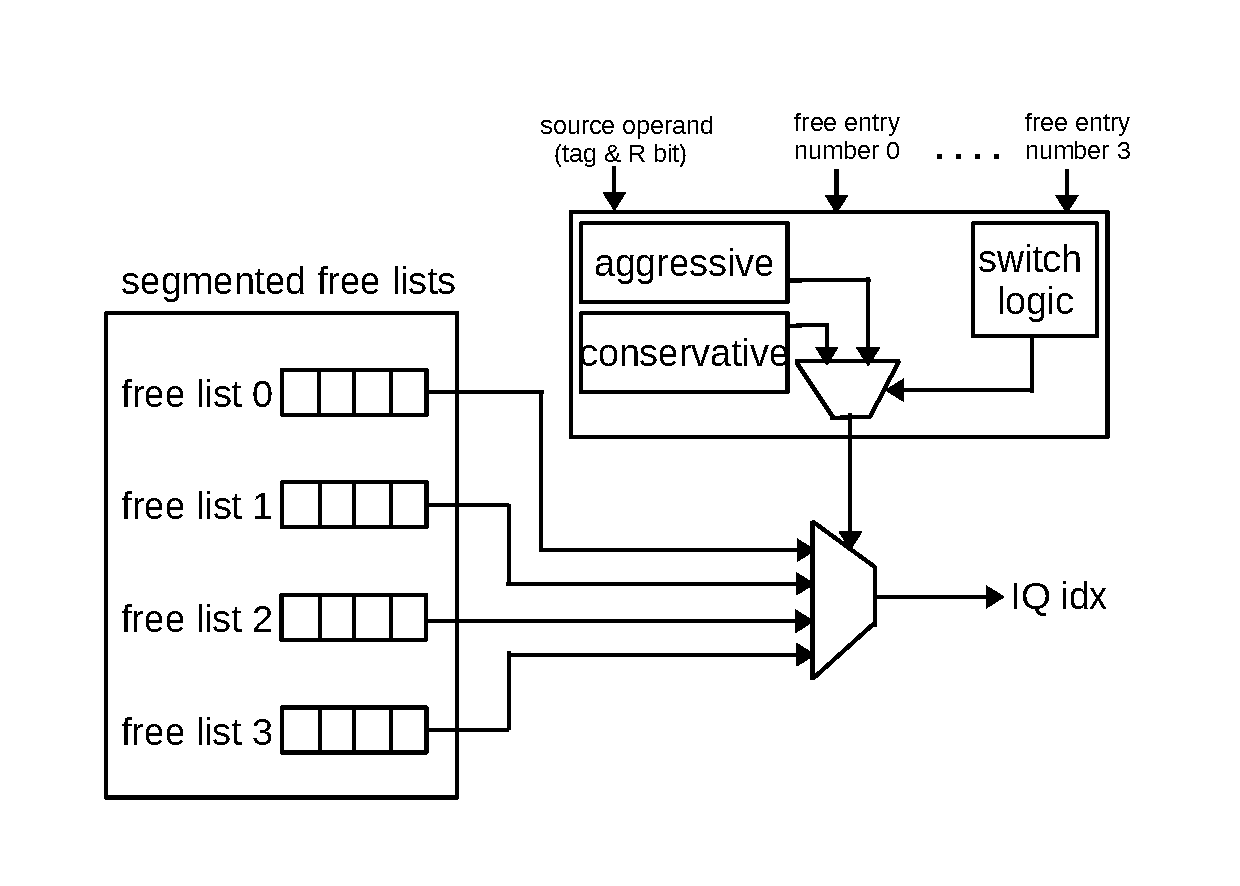
\includegraphics[keepaspectratio, scale=.8]{switch}
  \caption{SWITCH 方式におけるディスパッチエントリの決定回路}
  \label{fig:switch}
\end{figure}